\chapter{Commande des robots manipulateurs II: dynamique}

Ce chapitre présente des techniques de commande qui s'applique pour les systèmes robotisés où les entrées du système sont des forces ou couples produites par les actionneurs. Dans ce contexte, le système peut être modéliser comme un système d'équations différentielles non-linéaire d'ordre deux et être représentés par l'équation des manipulateurs décrite au chapitre \ref{sec:dynamic}.  Les vidéos suivants présentent une introduction, avec un point de vue graphique dans l'espace des phases, aux méthodes pour se contexte:

\video{Introduction à la commande des robots}{https://youtu.be/eL6i319X_w4}
\video{L'espace des phases}{https://youtu.be/eL6i319X_w4}
\video{Tour d'horizon des méthodes de commande dans l'espace des phases}{https://youtu.be/eL6i319X_w4}

Au lien suivant, une amorce de code pour tester des lois de commande sur un robot manipulateur à 2 DDL:
\colab{Testez votre loi de commande pour un manipulateur}{https://colab.research.google.com/drive/1bnJ9v5kHRFFhnNOZx-_Kcht2l5sTOHxr?usp=sharing}




\newpage
%%%%%%%%%%%%%%%%%%%%%%%%%%%%%%%%%%%%%%%%%%%%%%%
\section{Commande dé-localisée}
%%%%%%%%%%%%%%%%%%%%%%%%%%%%%%%%%%%%%%%%%%%%%%%

Dans certains situations, il est possible de traiter le problème de commande joint par joint avec des méthodes de commande classique comme des lois de commandes de type PID. Cette approche peut bien fonctionner surtout lorsque le système robotique a des actionneurs avec des grands ratios de réduction, ce qui minimise le couplage dynamique entre les divers DDL. Plus les effets inertiels et plus on désire suivre précisément des trajectoires dynamiques, moins ce type d'approche va être performante.

\colab{Simulation d'un manipulateur avec des PIDs }{https://colab.research.google.com/drive/1qaCNY2ohQIbC6dV2ZW4KY6FDM9NhJzH2?usp=sharing}

Détails à venir!


\newpage
%%%%%%%%%%%%%%%%%%%%%%%%%%%%%%%%%%%%%%%%%%%%%%%%%%%%%
\section{Commande avec la méthode du couple calculé}
%%%%%%%%%%%%%%%%%%%%%%%%%%%%%%%%%%%%%%%%%%%%%%%%%%%%%

La méthode du couple calculé consiste à utiliser les équations d'un modèle dynamique d'un système robotique pour déterminer les forces à appliquer pour obtenir une accélération cible. Il est ensuite possible de calculer cette accélération cible de sorte à converger vers la position ou trajectoire désirée.

\video{Méthode du couple calculé}{https://youtu.be/QuEhwAUxx5Y}


\subsection{Commande de l'accélération des joints}

Premièrement, si un système est pleinement actionné, il est possible d'imposé d'une accélération arbitraire dans l'espace des joints à un instant donné. Pour un système décrit par l'équation des manipulateurs:
%%%%%%%%%%%%%%%%%%%%%%%
\begin{align}
H(\col{q}) \col{\ddot{q}} + C(\col{q},\col{\dot{q}}) \col{\dot{q}} + d(\col{q}, \col{\dot{q}}) + \col{g}(\col{q}) = B(\col{q}) \col{u} 
\end{align}
%%%%%%%%%%%%%%%%%%%%%%%
si on définie une loi de commande avec une accélération référence $\col{\ddot{q}}_r$:
%%%%%%%%%%%%%%%%%%%%%%%
\begin{align}
\col{u} = B(\col{q})^{-1} \left[  H(\col{q}) \col{\ddot{q}}_r + C(\col{q},\col{\dot{q}}) \col{\dot{q}} + d(\col{q}, \col{\dot{q}}) + \col{g}(\col{q}) \right]
\end{align}
%%%%%%%%%%%%%%%%%%%%%%%
qui assume ici que la matrice $B$ est inversible, donc que le système est pleinement actionné. Alors si on substitut la loi de commande dans l'équation de la dynamique on obtient:
%%%%%%%%%%%%%%%%%%%%%%%
\begin{align}
H(\col{q}) \col{\ddot{q}} + C(\col{q},\col{\dot{q}}) \col{\dot{q}} + d(\col{q}, \col{\dot{q}}) + \col{g}(\col{q}) &= B(\col{q}) B(\col{q})^{-1} \left[  H(\col{q}) \col{\ddot{q}}_r + C(\col{q},\col{\dot{q}}) \col{\dot{q}} + d(\col{q}, \col{\dot{q}}) + \col{g}(\col{q}) \right]  \\
H(\col{q}) \col{\ddot{q}} &= H(\col{q}) \col{\ddot{q}}_r \\
\col{\ddot{q}} &= \col{\ddot{q}}_r
\end{align}
%%%%%%%%%%%%%%%%%%%%%%%
on obtient comme résultat que l'accélération du système peut être directement commandée. Comme illustré à la figure \ref{fig:computedtorque}, avec cette loi de commande, la relation entre la référence $\col{\ddot{q}}_r$ et la variable à contrôler $\col{q}$ est réduite à une relation linéaire, ici un double intégrateur. On réfère aussi parfois à cette méthode comme une boucle linéarisante.

%%%%%%%%%%%%%%%%%%%%%%%%%
\begin{figure}[htp]
	\centering
		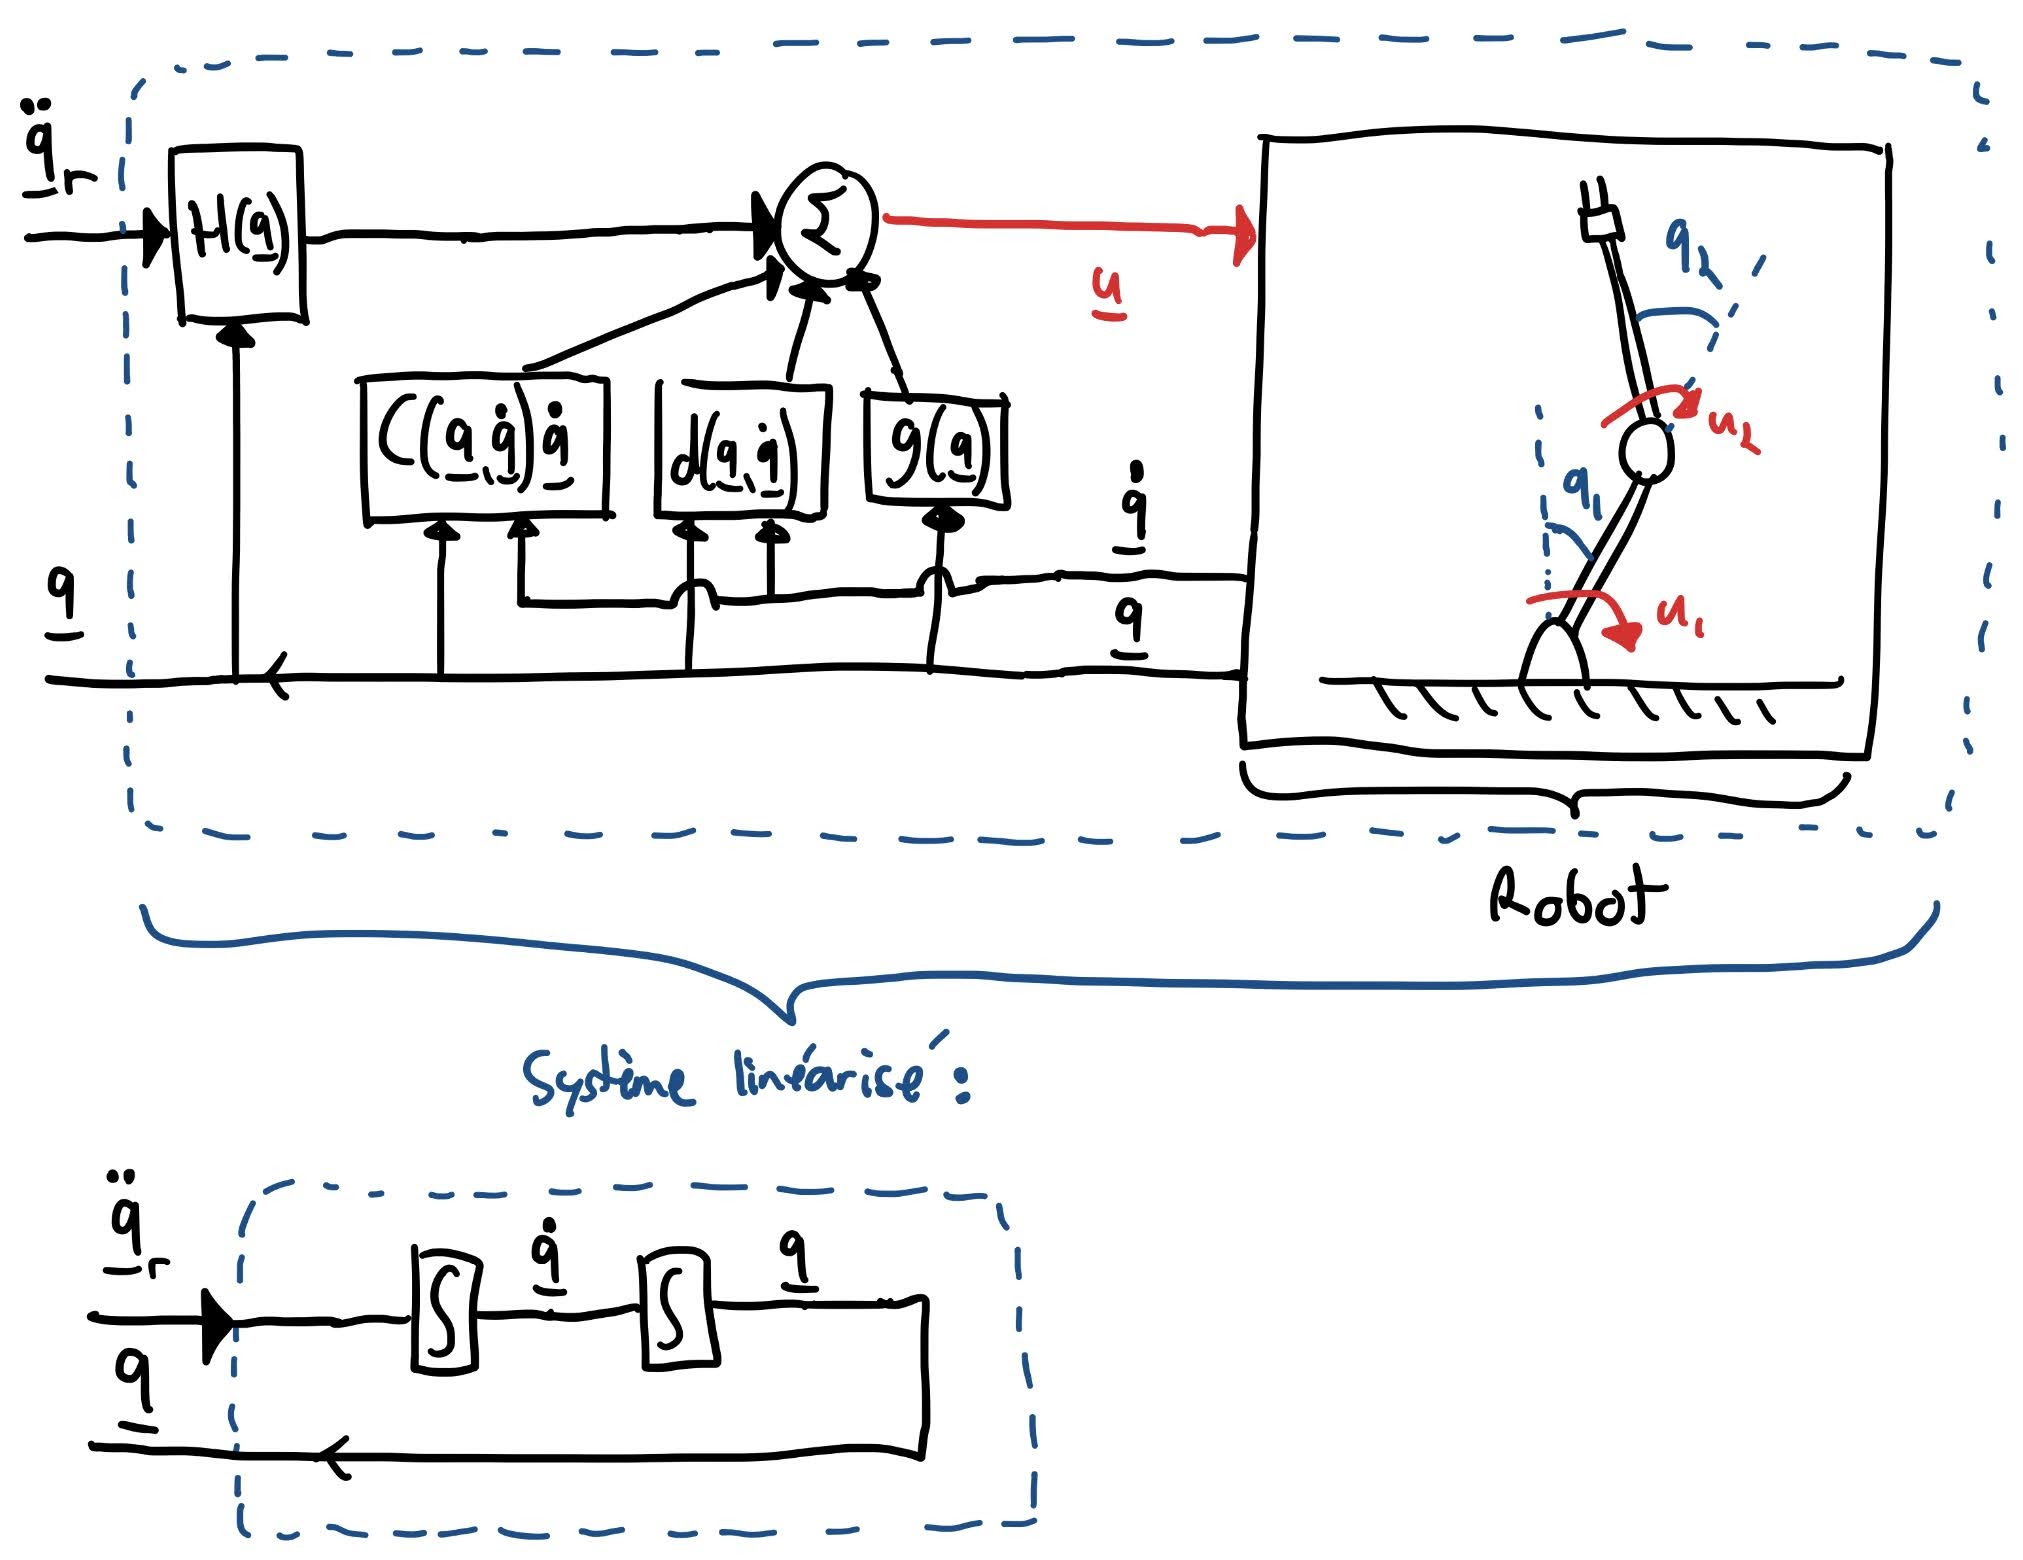
\includegraphics[width=0.75\textwidth]{fig/computedtorque.jpg}
	\caption{Couple calculé et boucle linéarisante. TODO Manque B}
	\label{fig:computedtorque}
\end{figure}
%%%%%%%%%%%%%%%%%%%%

\subsection{Suivi de trajectoire avec le couple calculé}

Lorsqu'on désire qu'un robot suivre une certaine trajectoire, il est possible de définir la référence d'accélération $\col{\ddot{q}}_r$ comme une fonction de la trajectoire cible pour obtenir que le robot va converger sur la trajectoire. Si une trajectoire cible est définie comme une fonction du temps pour les coordonnées $\col{q}$ et leur deux premières dérivées:
%%%%%%%%%%%%%%%%%%%%%%%
\begin{align}
\text{Trajectoire désirée: } \col{\ddot{q}}_d(t) \quad \col{\dot{q}}_d(t) \quad \col{q}_d(t)
\end{align}
%%%%%%%%%%%%%%%%%%%%%%%
alors si on définie la référence d'accélération par la loi de commande suivante:
%%%%%%%%%%%%%%%%%%%%%%%
\begin{align}
\col{\ddot{q}}_r = \col{\ddot{q}}_d + 2 \zeta w 
\underbrace{\left( \col{\dot{q}}_d - \col{\dot{q}}\right)}_{ \col{\dot{q}}_e}
+ w^2
\underbrace{\left( \col{q}_d - \col{q}\right)}_{ \col{q}_e}
\end{align}
%%%%%%%%%%%%%%%%%%%%%%%
puisqu'on obtient $\col{\ddot{q}} = \col{\ddot{q}}_r$ avec la méthode du couple calculé, en combinant cette définition pour $\col{\ddot{q}}_r$ on va obtenir:
%%%%%%%%%%%%%%%%%%%%%%%
\begin{align}
\underbrace{\left( \col{\ddot{q}}_d - \col{\ddot{q}} \right)}_{ \col{\ddot{q}}_e}
 + 2 \zeta w 
\underbrace{\left( \col{\dot{q}}_d - \col{\dot{q}}\right)}_{ \col{\dot{q}}_e}
+ w^2
\underbrace{\left( \col{q}_d - \col{q}\right)}_{ \col{q}_e} = 0
\label{eq:computedtorqueerrordynamic}
\end{align}
%%%%%%%%%%%%%%%%%%%%%%%
ce qui représente une équation de la dynamique pour l'erreur d'ordre 2 qui converge exponentiellement vers zéro si on choisi $w^2>0$ et $2 \zeta w > 0$, ce qui implique que la trajectoire du robot va converger sur la trajectoire désirée. 
%%%%%%%%%%%%%%%%%%%%%%%%%
\begin{figure}[htp]
	\centering
		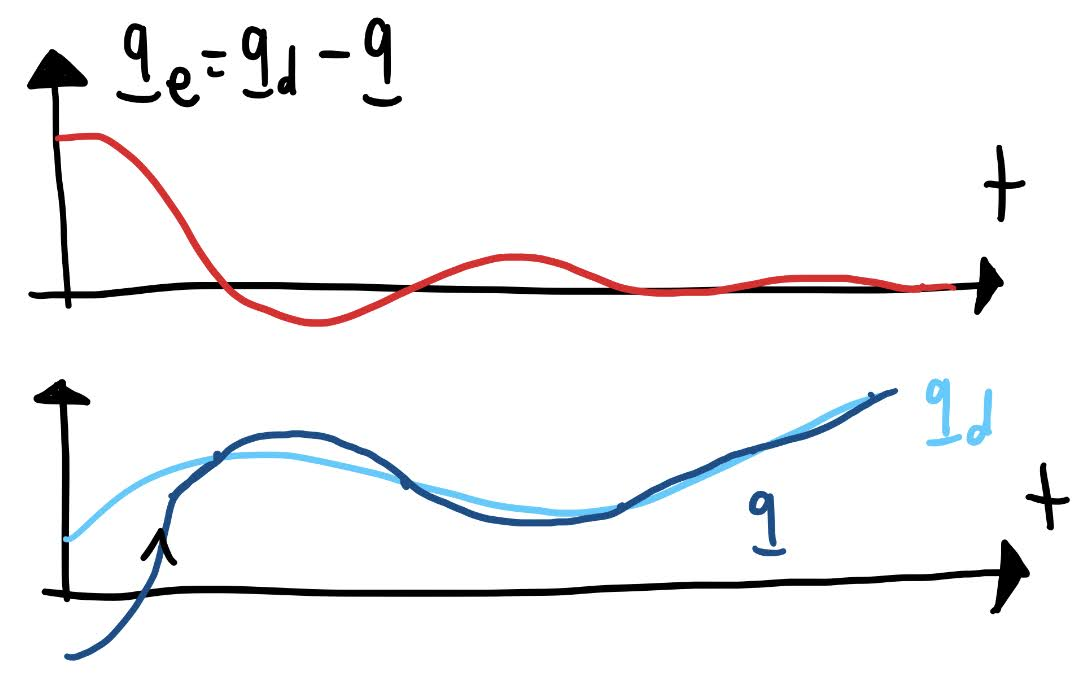
\includegraphics[width=0.50\textwidth]{fig/errordynamic.jpg}
	\caption{Dynamique de l'erreur et convergence sur la trajectoire}
	\label{fig:errordynamic}
\end{figure}
%%%%%%%%%%%%%%%%%%%%


On voit ici selon cette équation que ces paramètres dans la loi de commande ont été intégré de sorte qu'ils correspondent directement aux paramètres de fréquence naturelle et d'amortissement pour la forme standard d'une équation différentielle d'ordre deux. Ici $\zeta$ serait un paramètre de la loi de commande directement relié au dépassement et au temps d'établissement de l'erreur du système en boucle fermée et le $w$ au temps de monté et la bande passante du système en boucle fermée. De façon plus général, dans l'équation \eqref{eq:computedtorqueerrordynamic} le terme scalaire $w^2$ pourrait être remplacé par une matrice $K_p$ et le terme $2 \zeta w $ par une matrice $K_d$. Plutôt qu'avoir alors une dynamique d'erreur identique pour chaque DDL, on pourrait paramétrer des comportements plus varié. Par exemple, on pourrait choisir des matrices diagonales et les termes indépendants sur leur diagonale correspondraient à des valeurs de $w$ et $\zeta$ qui pourraient être choisi indépendemment pour chaque DDL du robot.
%%%%%%%%%%%%%%%%%%%%%%%%%
\begin{figure}[htp]
	\centering
		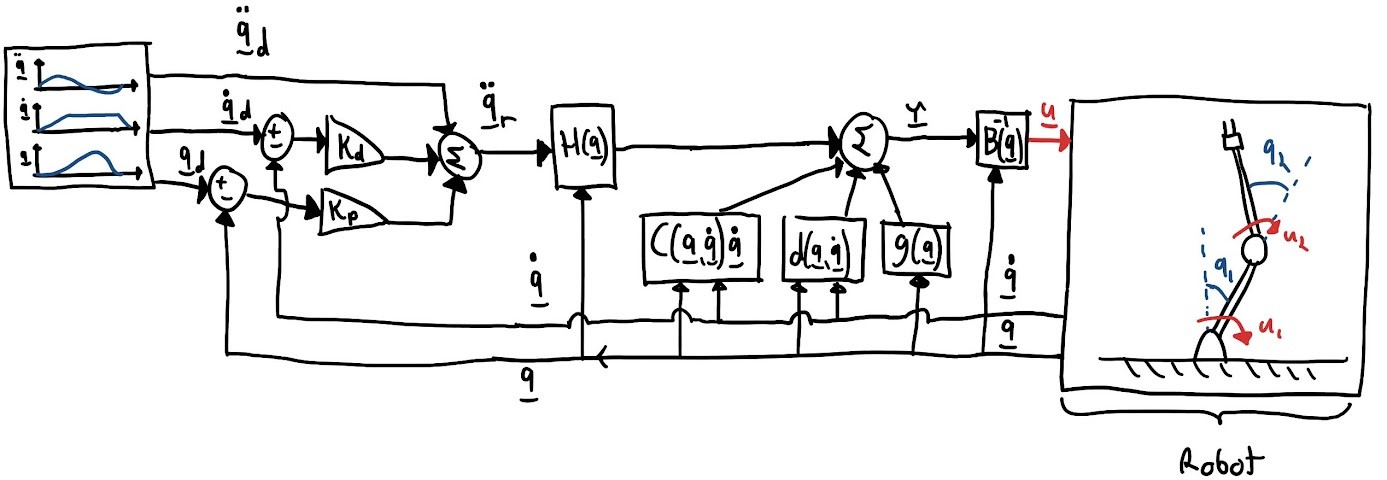
\includegraphics[width=0.99\textwidth]{fig/computedtorquetraj.jpg}
	\caption{Commande par couple calculé pour suivre une trajectoire. TODO manque B}
	\label{fig:computedtorquetraj}
\end{figure}
%%%%%%%%%%%%%%%%%%%%

Donc pour résumé, en assumant que notre modèle dynamique est parfait et que nous avons aussi des mesures exacte pour $\col{q}$ et $\col{\dot{q}}$, il est possible d'imposer une accélération instantanée $\col{\ddot{q}}_r$ arbitraire (si on ignore les limites des actionneurs pour le moment). Ensuite, connaissant la trajectoire cible $\col{q}_d(t)$ et ses dérivées d'ordre 1 et 2, il est possible d'imposer une accélération de sorte à avoir une erreur par rapport à la trajectoire $\col{q}_e(t)$qui tend vers zéro.







Si on regarde comment l'erreur est relié à une force demandée par la loi de commande, on peut interprété cette relation comme une matrice de rigidité, de même que pour un la relation avec la dérivé de l'erreur qui peut être interprété comme une matrice d'amortissement. Les autres termes qui ne sont pas relié à l'erreur ou l'accélération de la trajectoire cible ont tous comme rôle d'annuler des forces internes. Donc si on décortique la loi de commande, on peut regrouper les termes ansi:
%%%%%%%%%%%%%%%%%%%%%%%
\begin{align}
\col{u} &= B(\col{q})^{-1} \left[  H(\col{q}) \col{\ddot{q}}_r + C(\col{q},\col{\dot{q}}) \col{\dot{q}} + d(\col{q}, \col{\dot{q}}) + \col{g}(\col{q}) \right] \\
\col{u} &= B(\col{q})^{-1} \left[  H(\col{q}) \left( \col{\ddot{q}}_d + K_d  \col{\dot{q}}_e  + K_p \col{q}_e \right) + C(\col{q},\col{\dot{q}}) \col{\dot{q}} + d(\col{q}, \col{\dot{q}}) + \col{g}(\col{q}) \right] \\
\col{u} &= 
\underbrace{
\left[ B(\col{q})^{-1} H(\col{q})  \right] \, \col{\ddot{q}}_d 
}_{\text{Termes anticipatif}}
+ 
\underbrace{
\left[ B(\col{q})^{-1} H(\col{q}) K_d  \right] \,  \col{\dot{q}}_e 
+ 
\left[ B(\col{q})^{-1} H(\col{q}) K_p   \right] \, \col{q}_e 
}_{\text{Termes réactifs}}
+
\underbrace{
B(\col{q})^{-1} \left[ C(\col{q},\col{\dot{q}}) \col{\dot{q}} + d(\col{q}, \col{\dot{q}}) + \col{g}(\col{q}) \right]
}_{\text{Termes de compensation}}
\end{align}
%%%%%%%%%%%%%%%%%%%%%%%
et comparer à une loi de commande plus simple d'impédance dans le domaine des joints, présenté à la section \ref{sec:impcontrol}, qui est en fait aussi équivalent à utiliser des lois de commande de type proportionnelle-dérivée indépendantes pour chacun des joints. Premièrement, en plus de termes réactifs la méthode du couple calculé inclus plusieurs termes de compensation des forces internes du système, ainsi qu'un terme anticipatif si elle est utilisée pour faire du suivi de trajectoire. Ensuite, les termes réactifs ont une structure similaire, des vecteurs-colonnes d'erreur multiplient des matrices de gains. Toutefois, on remarque que dans le cas du couple calculé les matrices de gains $K_p$ et $K_d$ sont ajusté avec en étant multipliés par la matrice d'inertie $H(\col{q})$ et la matrice d'actionnement $B(\col{q})^{-1}$. Cet ajustement fait que nos gains dans les matrices $K_p$ et $K_d$ spécifient pas un lien linéaire avec un réaction en force, mais plutôt avec une réaction en accélération, pour laquelle on calcul la force nécessaire avec les matrice $H$ et $B$.


\subsection{Compensation de la friction}


%%%%%%%%%%%%%%%%%%%%%%%%%
\begin{figure}[htp]
	\centering
		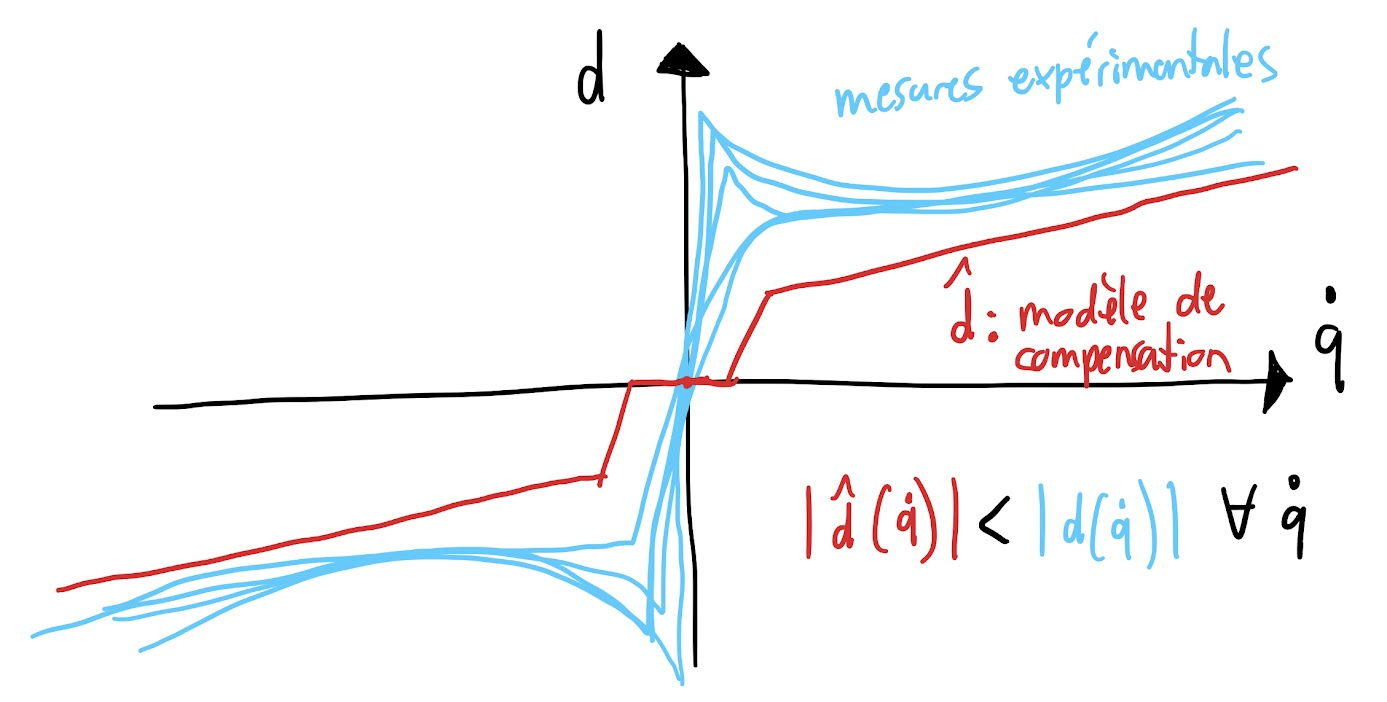
\includegraphics[width=0.99\textwidth]{fig/friction_compensation.jpg}
	\caption{Modèle de compensation de friction}
	\label{fig:friction_compensation}
\end{figure}
%%%%%%%%%%%%%%%%%%%%


\subsection{Suivi d'une trajectoire définie dans l'espace de la tâche}


\subsection{Limites de la méthode}


\subsection{Commande en impédance incluant les effets inertiels }

TODO voir notes manuscriptes alex 3 juillet 2022

\newpage
%%%%%%%%%%%%%%%%%%%%%%%%%%%%%%%%%%%%%%%%%%%%%%%
\section{Commande robuste}
%%%%%%%%%%%%%%%%%%%%%%%%%%%%%%%%%%%%%%%%%%%%%%%

La commande robuste est la science de gérer l'incertitude lors de la conception d'une loi de commande. Dans les sections précédentes, nous avions des lois de commande qui utilisaient divers propriétés du modèle cinématique et/ou dynamique du robot. Les démonstrations que ces lois de commande assumais alors que nos modèles utilisés dans les lois de commande étaient exacte. En pratique ce n'est jamais le cas, mais à divers degrés. Plus il y a d'incertitude dans un système et son comportement plus il y a intérêt à considérer cet aspect explicitement avec des méthodes de commande robuste.

\subsection{Approches pour modéliser l'incertitude}

%%%%%%%%%%%%%%%%%%%%%%%%%%%%%%%%
\begin{align}
H(\col{q}) \col{\ddot{q}} + C(\col{q},\col{\dot{q}}) \col{\dot{q}} + d(\col{q}, \col{\dot{q}}) + \col{g}(\col{q}) = B(\col{q}) \col{u}  + \col{w}
\end{align}
%%%%%%%%%%%%%%%%%%%%%%%%%%%%%%%%

\video{Grandes familles de méthodes de commande pour gérer l'incertitude}{https://youtu.be/hbZBF-OEZEw}

\subsection{Méthode du mode glissant}

La méthode du mode glissant est une approche de commande qui a comme principal attrait de pouvoir garantir la performance d'un système, malgré la présence de perturbations. En effet, si on connaît les valeurs maximums et mimimums qu'une perturbation peut prendre nous aurons une méthode pour sélectrionner des gains qui peuvent garantir la convergence.

\video{Commande avec le mode glissant}{https://youtu.be/0Asg81SBjmk}

Premièrement, 

%%%%%%%%%%%%%%%%%%%%%%%%%
\begin{figure}[htp]
	\centering
		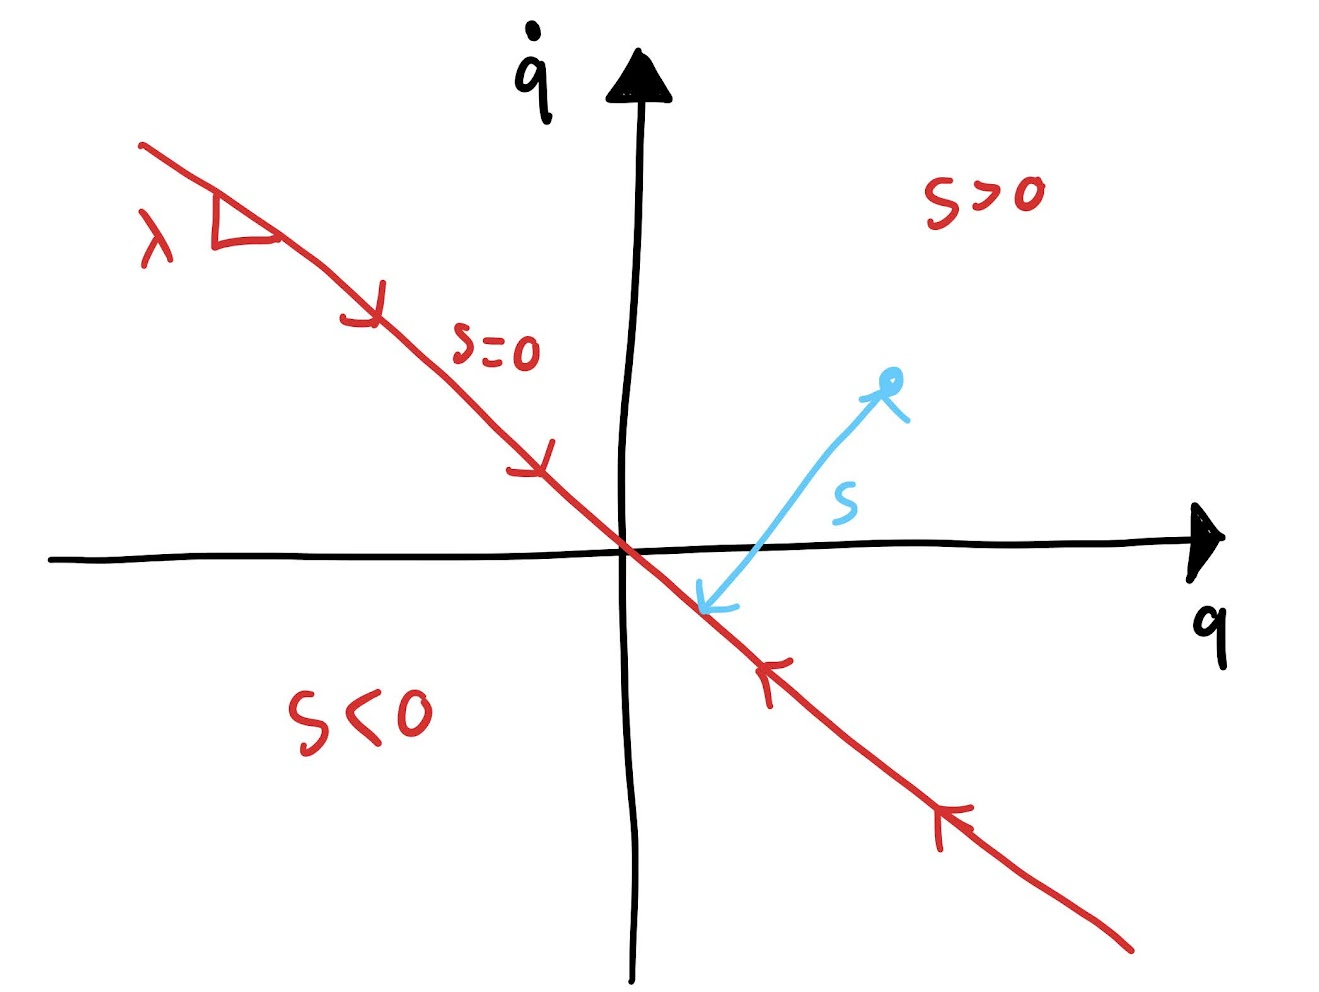
\includegraphics[width=0.99\textwidth]{fig/slidingmode.jpg}
	\caption{Surface glissante}
	\label{fig:slidingmode}
\end{figure}
%%%%%%%%%%%%%%%%%%%%


\newpage
%%%%%%%%%%%%%%%%%%%%%%%%%%%%%%%%%%%%%%%%%%%%%%%
\section{Commande adaptative}
%%%%%%%%%%%%%%%%%%%%%%%%%%%%%%%%%%%%%%%%%%%%%%%

\video{Exemple de loi de commande adaptative}{https://youtu.be/vmYjad6SOmU}


\section{Commande hybride en position et force}


\newpage
%%%%%%%%%%%%%%%%%%%%%%%%%%%%%%%%%%%%%%%%%%%%%%%
\section{Analyse de stabilité}
%%%%%%%%%%%%%%%%%%%%%%%%%%%%%%%%%%%%%%%%%%%%%%%

\video{Introduction à l'analyse de stabilité pour les systèmes non-linéaires}{https://youtu.be/q0Oqa5J3zEk}


\newpage
%%%%%%%%%%%%%%%%%%%%%%%%%%%%%%%%%%%%%%%%%%%%%%%
\section{Commande optimale}
%%%%%%%%%%%%%%%%%%%%%%%%%%%%%%%%%%%%%%%%%%%%%%%

\video{Exemple de loi de commande optimale pour un double intégrateur}{https://youtu.be/wKjEAXFvXlQ}

\video{Exemple de loi de commande optimale pour un pendule}{https://youtu.be/iUlkKdEK_dU}

\colab{Démo d'introduction aux méthodes de commande optimales}{https://colab.research.google.com/drive/1wXmlIqNGC2LrJkmyj56Y109b5ZDHVboq?usp=sharing}